\documentclass[a4paper, 12pt]{article}

\usepackage{cmap}
\usepackage[T2A]{fontenc}
\usepackage[utf8]{inputenc}

\usepackage[english, russian]{babel}

\usepackage{amsmath, amsfonts, amssymb, amsthm, mathtools}
\usepackage{icomma}

\usepackage{euscript}
\usepackage{mathrsfs}

\usepackage{graphicx}
\graphicspath{{images/}}

\author{Лепарский Роман Б01-003}
\title{Отчёт о выполнении лабораторной работы \\ \vspace{5mm} Построение диаграммы распределения сопротивлений большого количества резисторов}
\date{\today}

\begin{document}

\maketitle

\newpage

\section{Аннотация}

Целью работы является построение диаграмы распределения сопротивлений и сравнение её с результатами теоретических расчётов.

\section{Теоретические сведения}

При производстве резисторов реальное значение сопротивления может отличаться от номинального значения.
Эти отклонения соответствуют следующим критериям:

\begin{itemize}
	\item{Отклонения могут принимать непрерывный ряд значений.}
	\item{Отклонения одной величины но разного знака встречаются одинакого часто.}
	\item{Большие отклонения встречаются реже, чем малые.}
\end{itemize}

Это значит, что распределение сопротивлений подчиняется закону Гаусса:

\[	
f(x) = \frac{1}{\sigma \sqrt{2\pi}}\times e^{\frac{-(x-x_0)^2}{2\sigma ^2}}
\]

В качестве $x_0$ берется среднее арифметическое всех измерений, а в качестве $\sigma$ - среднее квадратичное отклонений. То есть:

\begin{align*}
	x_0 &= \frac{1}{N}\sum_{i=1}^N x_i \\
	\sigma^2 &= \frac{1}{N}\sum_{i=1}^N (x_i - x_0)^2
\end{align*}

Также, можно рассчитать вероятность попадения значения в интервал $(x_a, x_b)$ :

\[
P(x_a, x_b) = \int_{x_a}^{x_b} \frac{1}{\sigma \sqrt{2\pi}}\times e^{\frac{-(x-x_0)^2}{2\sigma ^2}} dx
\]

Табличные значения:

\begin{align*}
	&P(|x - x_0| \leq \sigma) \approx 0,68  \\
	&P(|x - x_0| \leq 2\sigma) \approx 0,95  \\
	&P(|x - x_0| \leq 3\sigma) \approx 0,995
\end{align*}

\section{Оборудование}

\begin{enumerate}
	\item {270 резисторов одинакового номинала}
	\item {Омметр}
\end{enumerate}

\section {Результаты измерений и обработка данных}

\subsection {Выполним измерения и заполним результаты в таблицу}

\begin{center}
\title{Результаты измерений} \\
\begin{tabular}{| c | c |}
	\hline      
	N &x, Ом      \\
	\hline      
	1 &$0,557$    \\
	\hline      
	2 &$0,560$    \\
	\hline      
	\dots &\dots  \\
	\hline
	269 &$0,555$  \\
	\hline      
	270 &$0,581$  \\
	\hline 
\end{tabular}
\end{center}

Результаты рассчётов:

\begin{align*}
	x_0 &= \frac{1}{270}\sum_{i=1}^{270} x_i = 0,562 \\ 
	\\
	\sigma &= \sqrt{\frac{1}{270}\sum_{i=1}^{270} (x_0 - x_i)^2} = 0,00973 
\end{align*}

\subsection{Построим диаграму}

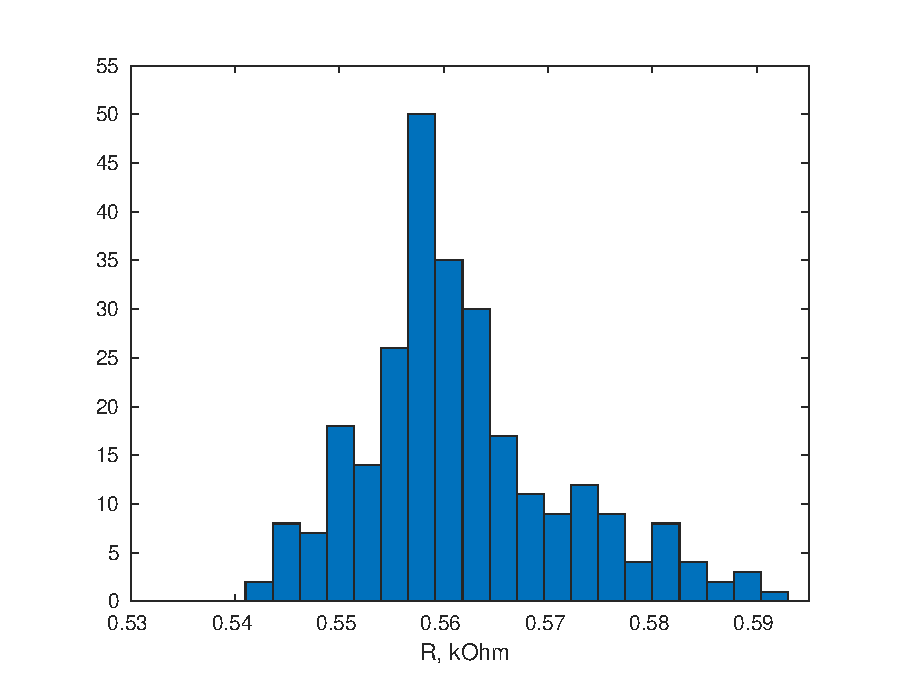
\includegraphics[scale = 0.7]{hist.eps}

\subsection{По вычисленным значениям $x_0$ и $\sigma$ построим график распределения Гаусса}

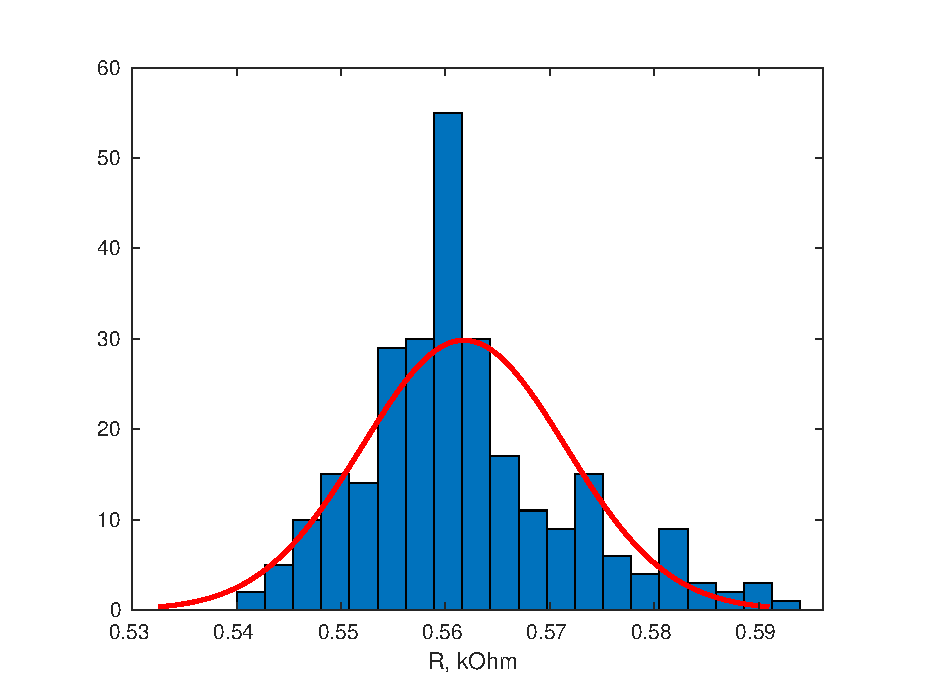
\includegraphics[scale = 0.7]{gauss.eps}

\subsection{Проверка теоретических вычислений}

Посчитаем количество резисторов, сопротивление которых попадает в интервалы $(x_0 - \sigma; x_0 + \sigma)$, $(x_0 - 2\sigma; x_0 + 2\sigma)$
и $(x_0 - 3\sigma; x_0 + 3\sigma)$.

\begin{align*}
N(|x_0 - x| \leq \sigma) &= 185 \Rightarrow P_{pr}(|x_0 - x| \leq \sigma) = \frac{185}{270} \approx 0,69   \\
N(|x_0 - x| \leq 2\sigma) &= 256 \Rightarrow P_{pr}(|x_0 - x| \leq 2\sigma) = \frac{256}{270} \approx 0,95 \\
N(|x_0 - x| \leq 3\sigma) &= 269 \Rightarrow P_{pr}(|x_0 - x| \leq 3\sigma) = \frac{269}{270} \approx 0,996
\end{align*}

\section{Вывод}

Несмотря на то, что диаграмма слабо похожа на кривую Гаусса (всилу малого количества измерений), вероятности попадения
значений в промежутки $(x_0 - \sigma; x_0 + \sigma)$, $(x_0 - 2\sigma; x_0 + 2\sigma)$
и $(x_0 - 3\sigma; x_0 + 3\sigma)$ почти совпадают с теоретическими рассчётами.

\end{document}